%\subsubsection{Desenvolvimento}

	%01 - Criação do database
	
	\par Com o ambiente de desenvolvimento pronto, começou de fato o
desenvolvimento. Primeiramente foi necessário criar o banco de dados no SGDB.
Este por sua vez foi criado com a ajuda do PgAdmin que é um software gráfico
para administração do SGDB, e que fornece uma interface gráfica de apoio para o
PotgreSql. Para criar era necessário ja estar com o PgAdmin aberto e conectado
a um servidor de banco de dados que neste caso era em servidor local como pode
ser visto na Figura \ref{fig:desws}.

	\begin{figure}[h!]
		\centerline{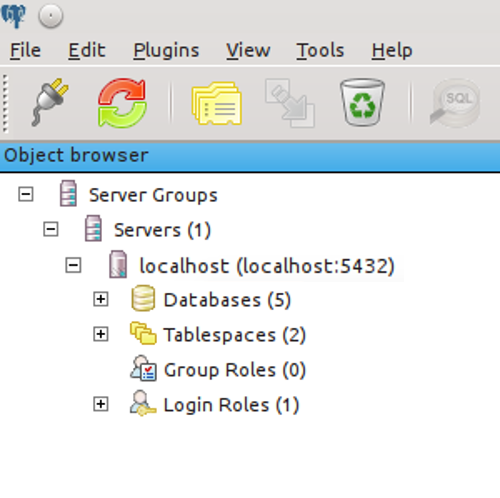
\includegraphics[scale=1]{./imagens/2_q_metodologico/4_procedimentos_resultados/43_webservice/432_desenvolvimento/desws.png}}
		\caption[Servidor de banco de dados local no PgAdmin]{Servidor de banco de
		dados local no PgAdmin.
			\textbf{Fonte:}Elaborado pelos autores.}
		\label{fig:desws}
	\end{figure}
	
	\pagebreak
	
	\par Para a efetiva criação do banco de dados era necessário clicar com o
botão direito do \textit{mouse}, sobre a opção \textbf{Databases -> New
Database\ldots} no PgAdmin, apresentada na Figura \ref{fig:desws1}.

	\begin{figure}[h!]
		\centerline{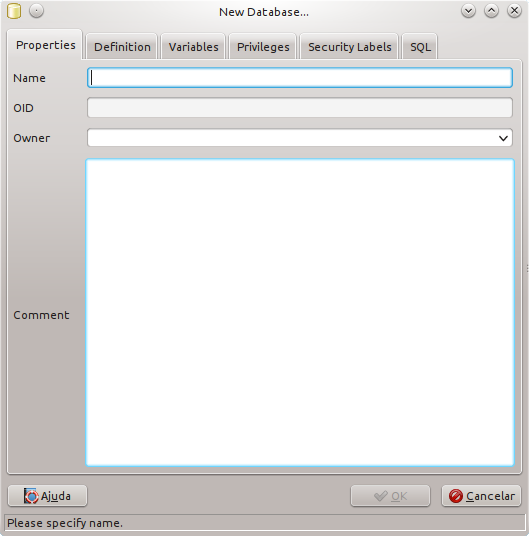
\includegraphics[scale=0.8]{./imagens/2_q_metodologico/4_procedimentos_resultados/43_webservice/432_desenvolvimento/desws1.png}}
		\caption[Opção \textit{New Database\ldots}]{Opção \textit{New Database\ldots}.
			\textbf{Fonte:}Elaborado pelos autores.}
		\label{fig:desws1}
	\end{figure}

	\pagebreak
	
	\par Em seguida foi necessário preencher o dados da janela apresentada, como
está apresentado na Figura \ref{fig:desws2}.
	
	\begin{figure}[h!]
		\centerline{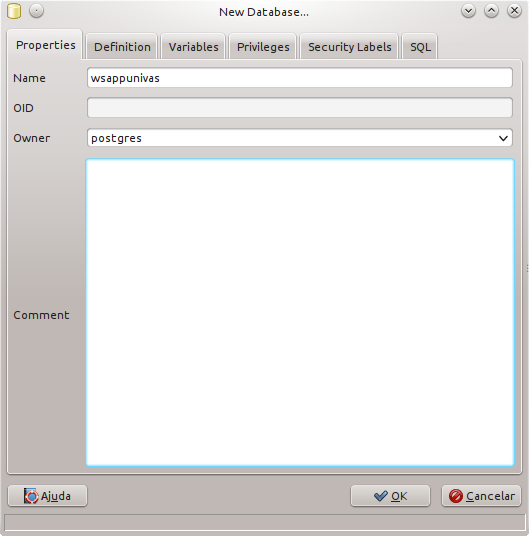
\includegraphics[scale=1]{./imagens/2_q_metodologico/4_procedimentos_resultados/43_webservice/432_desenvolvimento/desws2.png}}
		\caption[Tela \textit{New Database\ldots}]{Tela \textit{New Database\ldots}.
			\textbf{Fonte:}Elaborado pelos autores.}
		\label{fig:desws2}
	\end{figure}
	
	\pagebreak

	\par Como pode ser visto foram preenchidos os campos nome e usuário . O campo
nome se refere ao nome do banco de dados que foi definido com
\texttt{wsappunivas}, e usuário, o responsável pelo banco de dados, que para
este caso foi usuário padrão do SGDB, que é o \texttt{postgres}. Além destas
configurações mais nenhuma foi necessária. O banco de dados foi criado, porém
sua estrutura não foi definida, pois como será visto mais adiante o Hibernate,
possui um mecanismo, que com algumas configurações, permite a estruturação do
banco de dados, de acordo com o mapeamento objeto-relacional e de acordo com a
evolução do projeto. Isto permitirá mudanças na estrutura do banco de dados e
suas tabelas, e até mesmo eventuais correções.
	
	%02 - Início do projeto web no eclipse;
	\par Em seguida foi criado um projeto do tipo Dynamic Web Project no
Eclipse. Para proceder com a criação de um novo projeto deste tipo no Eclipse, é
necessário acessar na IDE, a opção \textbf{File -> New-> Dynamic Web Project}
como pode ser visto na figura \ref{fig:desws3}.

	
	\begin{figure}[h!]
		\centerline{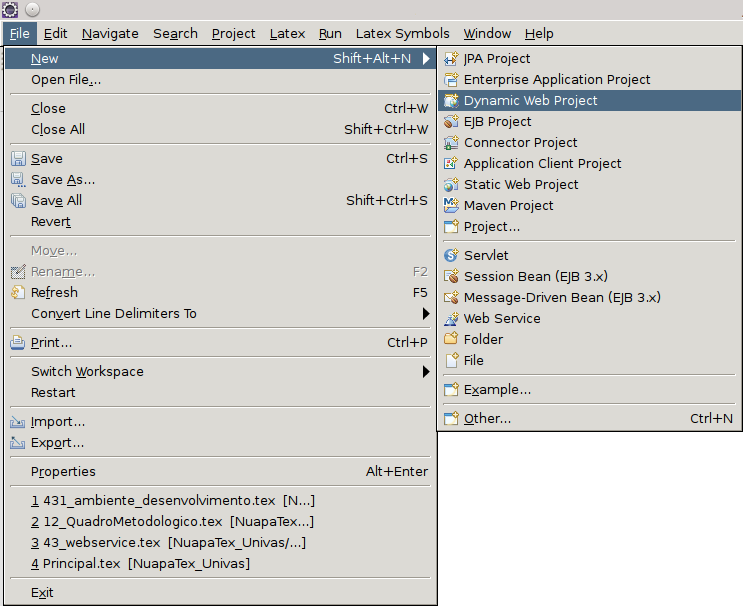
\includegraphics[scale=0.8]{./imagens/2_q_metodologico/4_procedimentos_resultados/43_webservice/432_desenvolvimento/desws3.png}}
		\caption[Tela \textit{New Database\ldots}]{Tela \textit{New Database\ldots}.
			\textbf{Fonte:}Elaborado pelos autores.}
		\label{fig:desws3}
	\end{figure}
	
	\pagebreak
	
 	\par Em seguida foi apresentada uma tela para o preenchimento de alguns dados
 requeridos para a criação do projeto. Destas informações somente foi preenchido
 o nome do projeto. As outras informações continuaram sendo as que vem por
 padrão da IDE. A janela apresentada e as informações preenchidas podem ser
 vistas na Figura \ref{fig:desws4}.

	\begin{figure}[h!]
		\centerline{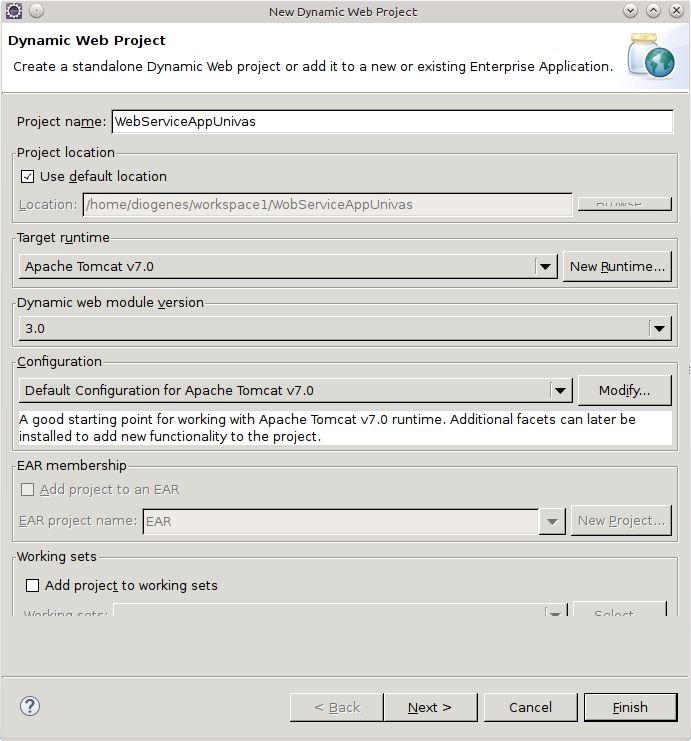
\includegraphics[scale=0.8]{./imagens/2_q_metodologico/4_procedimentos_resultados/43_webservice/432_desenvolvimento/desws4.png}}
		\caption[Tela para criação de um novo projeto no Eclipse]{Tela para criação de um novo projeto no Eclipse.
			\textbf{Fonte:}Elaborado pelos autores.}
		\label{fig:desws4}
	\end{figure}
	
	\pagebreak
	
	
	\par Na próxima janela apresentada, que têm por função configurar a pasta de
códigos do projeto manteve-se a configuração apresentada pela IDE, como mostra
a Figura \ref{fig:desws5}.

	\begin{figure}[h!]
		\centerline{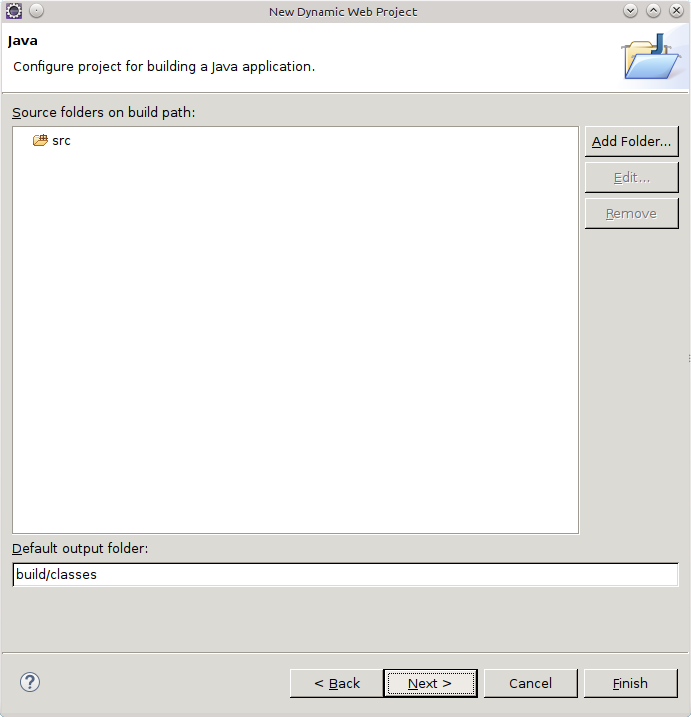
\includegraphics[scale=0.8]{./imagens/2_q_metodologico/4_procedimentos_resultados/43_webservice/432_desenvolvimento/desws5.png}}
		\caption[Tela para criação de um novo projeto no Eclipse]{Tela para criação de um novo projeto no Eclipse.
			\textbf{Fonte:}Elaborado pelos autores.}
		\label{fig:desws5}
	\end{figure}
	
	\pagebreak
	
	\par Na sequencia, na tela que foi apresentada era necessário preencher o
campo \textbf{Context root:} com o contexto principal da aplicação web que
acabou mantendo o próprio nome da aplicação. Além disso foi marcado a opção
\textbf{Generate web.xml deployment descriptor}, para que ao criar o projeto, a
própria IDE criasse o arquivo \texttt{web.xml}, arquivo responsável por algumas
configurações da aplicação web. Esta tela esta apresentada na Figura
\ref{fig:desws6}.

	\begin{figure}[h!]
		\centerline{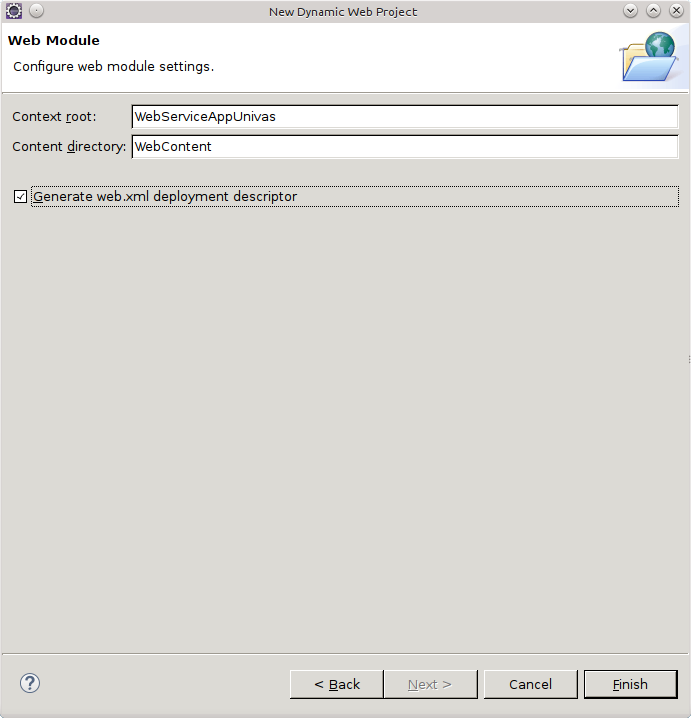
\includegraphics[scale=0.8]{./imagens/2_q_metodologico/4_procedimentos_resultados/43_webservice/432_desenvolvimento/desws6.png}}
		\caption[Tela para criação de um novo projeto no Eclipse]{Tela para criação de um novo projeto no Eclipse.
			\textbf{Fonte:}Elaborado pelos autores.}
		\label{fig:desws6}
	\end{figure}
	
	\pagebreak

	%03 - Mapeamento orm;	
		%	->Criação do pacote

	\par Após este passo foi concluído a criação do projeto, e já era possível
iniciar os trabalhos com a camada de persistência de dados do projeto. Para
este propósito, primeiramente foi criado um pacote, onde ficaram contidas as
classes que representam as entidades do ORM. Para a criação do pacote foi
necessário clicar com o botão direito do mouse sobre o projeto e acessar a opção
\textbf{New -> Package}, como pode ser visto na Figura \ref{fig:desws7}.

	\begin{figure}[h!]
		\centerline{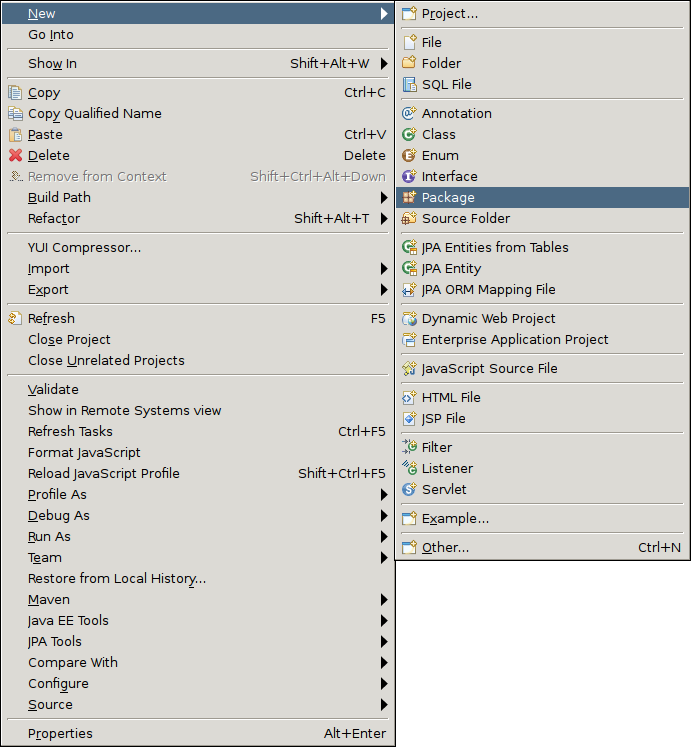
\includegraphics[scale=0.8]{./imagens/2_q_metodologico/4_procedimentos_resultados/43_webservice/432_desenvolvimento/desws7.png}}
		\caption[Tela para criação de um novo projeto no Eclipse]{Tela para criação de um novo projeto no Eclipse.
			\textbf{Fonte:}Elaborado pelos autores.}
		\label{fig:desws7}
	\end{figure}
	
	\pagebreak 
	
	\par Em seguida foi apresentada a janela New Java Package, para a criação de
um novo pacote mostrada na Figura \ref{fig:desws8}. O pacote recebeu o nome de
"\texttt{br.edu.univas.restapiappunivas.model}", pois nele estão contidas as
classes que fazem parte do modelo de negócios da aplicação. Este pacote foi
criado visando a divisão das responsabilidades internas no projeto, além de
contribuir positivamente com a organização do mesmo.

	\begin{figure}[h!]
		\centerline{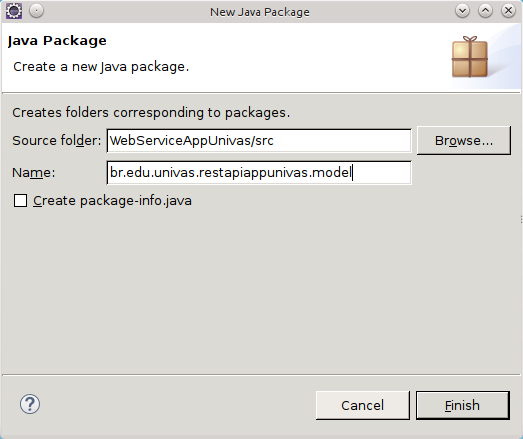
\includegraphics[scale=0.8]{./imagens/2_q_metodologico/4_procedimentos_resultados/43_webservice/432_desenvolvimento/desws8.png}}
		\caption[Tela para criação de um novo projeto no Eclipse]{Tela para criação de um novo projeto no Eclipse.
			\textbf{Fonte:}Elaborado pelos autores.}
		\label{fig:desws8}
	\end{figure}
	
	\pagebreak
		
		%	->Criação das classes
	\par Com este pacote criado, ja era possível criar as classes do ORM. Foi
criada primeiramente a classe \texttt{Student.java}. Para a criação desta classe
foi necesário clicar com o botão direito do \textit{mouse} sobre o projeto e
navegar até a opção \textbf{New -> Class} como pode ser visto na Figura
\ref{fig:desws9}. 

	\begin{figure}[h!]
		\centerline{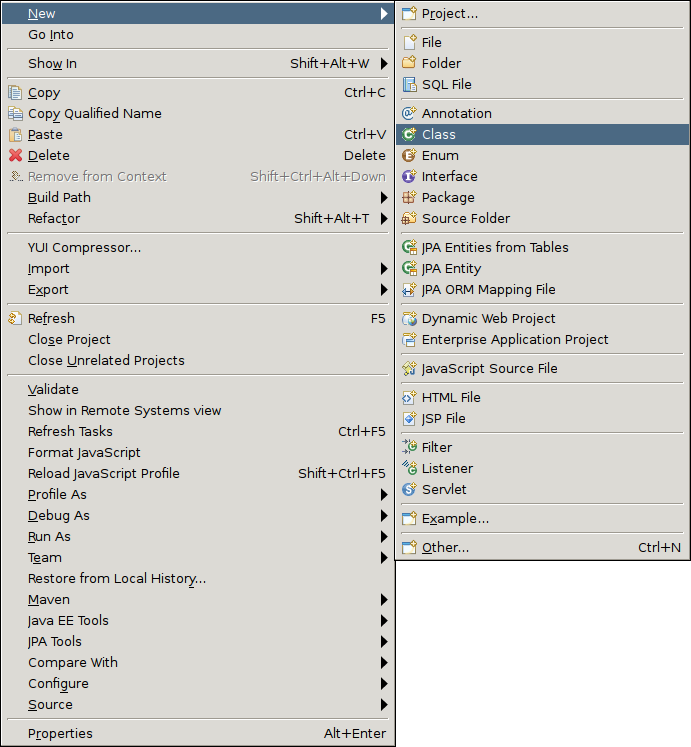
\includegraphics[scale=0.8]{./imagens/2_q_metodologico/4_procedimentos_resultados/43_webservice/432_desenvolvimento/desws9.png}}
		\caption[Sem legenda]{Sem legenda.
			\textbf{Fonte:}Elaborado pelos autores.}
		\label{fig:desws9}
	\end{figure}
	
	\pagebreak


	\par Em seguida foi apresentada uma janela chamada New Java Class. Nesta
janela somente foi necessário preencher o campo \textbf{Name:} que representa o
nome da classe que está sendo criada.
	
	
	
	 \begin{figure}[h!]
		\centerline{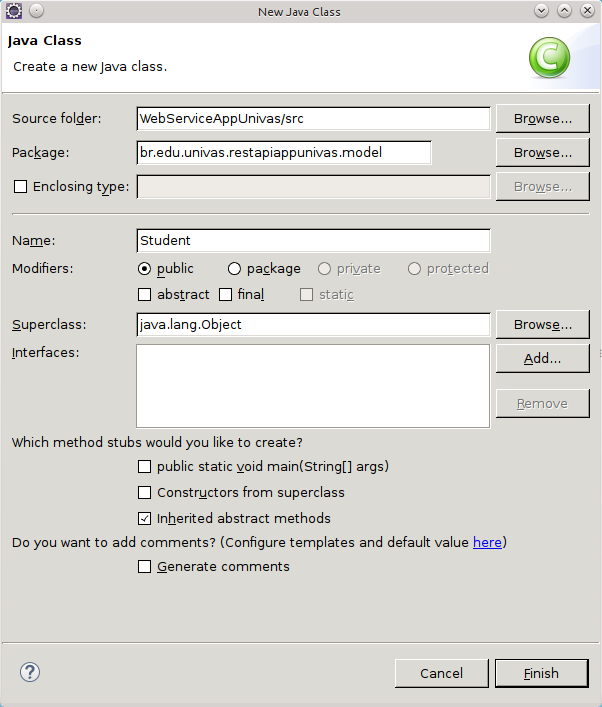
\includegraphics[scale=0.8]{./imagens/2_q_metodologico/4_procedimentos_resultados/43_webservice/432_desenvolvimento/desws10.png}}
		\caption[Sem legenda]{Sem legenda.
			\textbf{Fonte:}Elaborado pelos autores.}
		\label{fig:desws10}
	\end{figure}
	
	\pagebreak

	\par Esta classe foi definida para representar as informações referente aos
alunos. o código da classe pode ser visto na Figura \ref{fig:desws11}. 
	
	
	\begin{figure}[h!]
		\begin{lstlisting} [style=custom_Java]	
	package br.edu.univas.restapiappunivas.model;
	/**
	 *imports omitidos
	 */
	
	@Entity
	@Table(name = "student")
	public class Student {
	
		@Id
		@SequenceGenerator(name = "id_student", sequenceName = "seq_id_student",
			allocationSize = 1) 
		@GeneratedValue(generator = "id_student", strategy = GenerationType.IDENTITY)
		@Column(name = "id_student", nullable = false)
		private Long idStudent;
	
		@Column(name = "id_external", nullable = false)
		private Long idDatabaseExternal;
	
		@Column(length = 100, nullable = false)
		private String name;
	
		@Column(length = 100, nullable = false)
		private String email;
	
		@OneToMany(mappedBy="student", fetch = FetchType.EAGER)
		private List<Event> events;
	
		@OneToOne(optional = false, fetch = FetchType.LAZY)
		@JoinColumn(name = "id_user")
		private User user;
	
		/**
		 * Omitidos todos Getters e Setters
		 */
	
		@Override
		public int hashCode() {
			/**
			 * Omitido
			 */
		}
	
		@Override
		public boolean equals(Object obj) {
			/**
			 * Omitido
			 */
		}
	
	}
\end{lstlisting}
		\caption[Sem legenda]{Sem legenda.
			\textbf{Fonte:}Elaborado pelos autores.}
		\label{fig:desws11}
	\end{figure}
	
	\pagebreak
	
	\par É válido lembrar esta classe possui anotações para que possa ser
reconhecida como uma entidade do JPA, e assim persistida no banco de dados
quando necessário. Além disso estas anotações possuem outras finalidades
específicas. A seguir estão listadas todas as anotações  que foram usadas na
classe \texttt{Student.java} e nas outras classes que fazem parte do mapeamento
objeto relacional da aplicação.

	\begin{itemize}
	  \item \texttt{@Entity}: esta anotação foi necessária para que esta classe
	  pudesse ser reconhecida como uma entidade do JPA e assim persistida no banco
	  de dados;
	  \item \texttt{@Table}: anotação que possui algumas configurações relativas a
	  tabela no banco de dados, a qual esta entidade representa, no caso da classe'
	  mostrada anteriormente é configurado o nome da tabela;
	  \item \texttt{@Id}: esta anotação fica sobre o atributo que representa a
	  chave primária no banco de dados;
	  \item \texttt{@SequenceGenerator}: esta anotação define qual será o modo com
	  que a chave primaria será incrementada.
	  \item \texttt{@Column}: define algumas propriedades do campo da tabela do
	  banco de dados, o qual o atributo que ele anota representa. Estas
	  configuraçãoes podem são:
		  	\begin{itemize}
		    	\item \texttt{name}: muda o nome do campo;
		    	\item \texttt{length}: determina o tamanho em caracteres que o campo
		    	aceitará;
		    	\item \texttt{nullable}: define se o preenchimento do campo é obrigatório;
		    	\item \texttt{unique}: este atributo define se o campo aceitará valores
		    	únicos;
		    \end{itemize}
	  \item \texttt{@OneToMany}: representa um relacionamento um-para-muitos no
	  banco de dados. Anotam coleções de outras entidades;
	  \item \texttt{@ManyToOne}: representa um relacionamento
	  muitos-para-um no banco de dados. Este é a contraparte da anotação
	  um-para-muitos;
	  \item \texttt{@OneToOne}: representa um relacionamento um-para-um no banco de
	  dados.
\end{itemize}
 
	\par Esta classe faz parte do mecanismo de persistêcia de dados e é
simplesmente um  pojo ou seja, um objeto  simples que contêm somente atributos
privados e os métodos \textit{getters} e \textit{setters} que servem apenas
para encapsular estes atributos. Além desta classe, foram criadas outras com os
mesmos propósitos. Estas classes tinham a mesma finalidade da anterior, porém
com pequenas diferenças no que diz respeito à atributos, metodos e anotações.
Estas classes representam, de maneira individual, as tabelas no banco de dados.
As classes podem ser vistas na Figura \ref{fig:desws12}.
	
	
	\begin{figure}[h!]
		\centerline{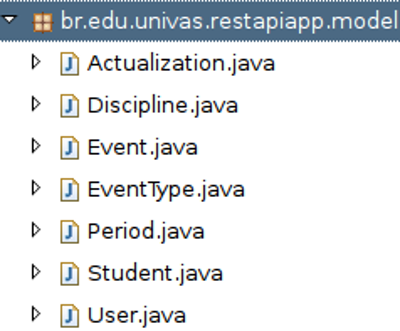
\includegraphics[scale=0.8]{./imagens/2_q_metodologico/4_procedimentos_resultados/43_webservice/432_desenvolvimento/desws12.png}}
		\caption[Sem legenda]{Sem legenda.
			\textbf{Fonte:}Elaborado pelos autores.}
		\label{fig:desws12}
	\end{figure}
	
	\pagebreak

	%04 - HashCode e equals
	\par E por fim, para cada classe que representa uma entidade, foi necessário
implementar os métodos \texttt{hashCode} e \texttt{equals}, para que estas
pudessem facilmente ser comparadas e diferenciadas em relação aos seus
valores, haja visto que cada instância destas classes representa um registro
no banco de dados. A própria IDE provê uma forma facíl para criar este métodos,
bastando para isso clicar com o botão direito do mouse sobre o código da classe
e escolher a opção \textbf{Source -> Generate hashCode() and equals()\ldots}
como pode ser visto na Figura \ref{fig:desws13}.

	\begin{figure}[h!]
		\centerline{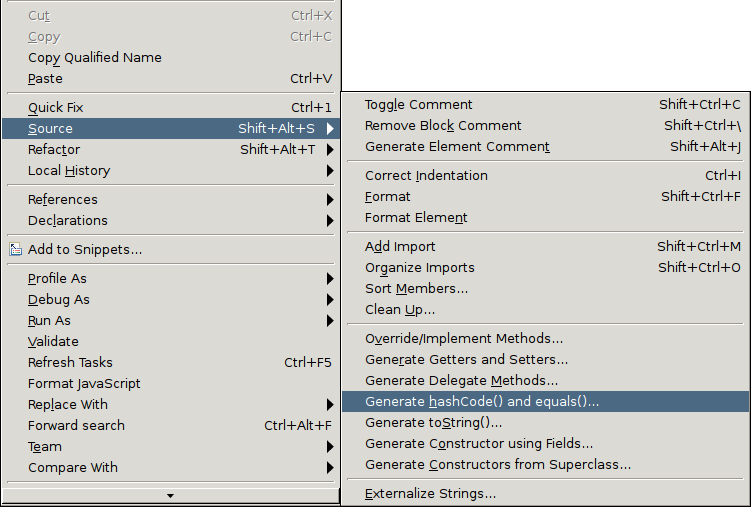
\includegraphics[scale=0.8]{./imagens/2_q_metodologico/4_procedimentos_resultados/43_webservice/432_desenvolvimento/desws13.png}}
		\caption[Sem legenda]{Sem legenda.
			\textbf{Fonte:}Elaborado pelos autores.}
		\label{fig:desws13}
	\end{figure}
	
	\pagebreak

	\par Os métodos \texttt{hashCode} e \texttt{equals} da
classe \texttt{Student.java} foram implementados usando o atributo id pode ser
visto na imagem
	
	\begin{figure}[h!]
		%implementação dos métodos hashCode() e equals()

\begin{lstlisting} [style=custom_Java] 	
	...
	
	@Override
	public int hashCode() {
		final int prime = 31;
		int result = 1;
		result = prime * result
				+ ((idStudent == null) ? 0 : idStudent.hashCode());
		return result;
	}

	@Override
	public boolean equals(Object obj) {
		if (this == obj)
			return true;
		if (obj == null)
			return false;
		if (getClass() != obj.getClass())
			return false;
		Student other = (Student) obj;
		if (idStudent == null) {
			if (other.idStudent != null)
				return false;
		} else if (!idStudent.equals(other.idStudent))
			return false;
		return true;
	}
	...
\end{lstlisting}

		\caption[Sem legenda]{Sem legenda.
			\textbf{Fonte:}Elaborado pelos autores.}
		\label{fig:desws11}
	\end{figure}
	
	
	%05 - Configuração do persistence.xml
	\par Em seguida à criação das entidades, foi necessário configurar o arquivo
\texttt{persistence.xml} que fica dentro do \textit{classpath} do projeto
Java ou seja, dentro da mesma pasta onde estão contidos pacotes do
projeto. Este arquivo é extremamente importante, pois é nele que estão todas
as configurações relativas à conexão com o banco de dados, configurações
referentes ao Dialeto SQL que vai ser usado para as consultas e configurações
referentes ao \textit{persistence unit} que é o conjunto de classes mapeadas
para o banco de dados.	O arquivo \texttt{persistence.xml} está exposto na
Figura \ref{fig:qm11}.

	\begin{figure}[h!]
		%persistence.xml
\begin{lstlisting} [style=custom_XML]
<?xml version="1.0" encoding="UTF-8"?>
<persistence version="2.1"
	xmlns="http://xmlns.jcp.org/xml/ns/persistence" 
	xmlns:xsi="http://www.w3.org/2001/XMLSchema-instance"
	xsi:schemaLocation="http://xmlns.jcp.org/xml/ns/persistence
	http://xmlns.jcp.org/xml/ns/persistence/persistence_2_1.xsd">
		<persistence-unit name="WsAppUnivas" transaction-type="RESOURCE_LOCAL">
					<provider>
						org.hibernate.jpa.HibernatePersistenceProvider
					</provider>
					<properties>
								<property name="javax.persistence.jdbc.url"
									value="jdbc:postgresql://localhost:5432/wsappunivas" />
								<property name="javax.persistence.jdbc.user" 
									value="postgres" />
								<property name="javax.persistence.jdbc.password" 
									value="omitido" />
								<property name="javax.persistence.jdbc.driver" 
									value="org.postgresql.Driver" />
								<property name="hibernate.dialect" 
									value="org.hibernate.dialect.PostgreSQLDialect" />
								<property name="hibernate.format_sql" 
									value="true" />
								<property name="hibernate.temp.use_jdbc_metadata_defaults"
									value="false" />
								<property name="hibernate.show_sql" 
									value="true" />
								<property name="hibernate.hbm2ddl.auto" 
									value="create" />
					</properties>
		</persistence-unit>
</persistence>
\end{lstlisting}
		\caption[Arquivo \texttt{persistence.xml}]{Arquivo \texttt{persistence.xml}.
		\textbf{Fonte:}Elaborado pelos autores.}
		\label{fig:qm11}
	\end{figure}
	
	%06 - Confecção JpaUtil.java
	\par Em seguida à confecção do \texttt{persistence.xml} foi criada a
classe \texttt{JpaUtil} que está representada na Figura \ref{fig:qm12}.
Esta classe é responsável por criar uma \texttt{EntityManagerFactory}. Este por
sua vez é uma  fábrica de instâncias de \texttt{EntityManager} é que um
\textit{persistence unit} ou unidade de persistência. Essa classe tem a
responsabilidade de prover um modo de comunicação entre a aplicação e o banco
de dados. No entanto a classe \texttt{JpaUtil} cria uma única instância de
\texttt{EntityManagerFactory}, que é responsável por disponibilizar e gerenciar
as instâncias de \texttt{EntityManager} de acordo com a necessidade da
aplicação.
	
	\begin{figure}[h!]
		%classe JpaUtil.java

\begin{lstlisting} [style=custom_Java] 	
package br.edu.univas.restapiappunivas.util;

import javax.persistence.EntityManager;
import javax.persistence.EntityManagerFactory;
import javax.persistence.Persistence;

public class JpaUtil {
	private static EntityManagerFactory factory;

	static {
		factory = Persistence.createEntityManagerFactory("WsAppUnivas");
	}

	public static EntityManager getEntityManager() {
		return factory.createEntityManager();
	}

	public static void close() {
		factory.close();
	}

}
	
\end{lstlisting}
		\caption[Classe \texttt{JpaUtil.java}]{Classe \texttt{JpaUtil.java}.
		\textbf{Fonte:}Elaborado pelos autores.}
		\label{fig:qm12}
	\end{figure}

	\pagebreak
		
	\par Em seguida à construção das classes que fazem a parte da persistência de
dados, foi desenvolvido a parte de disponibilização de serviços
RESTful, fazendo uso do \textit{framework} Jersey. Com isso
pode-se construir a classe que representa o primeiro serviço do
\textit{webservice}, que é a classe \texttt{Alunos}. Essa classe representa um
contexto REST, e portanto, dispõe de alguns recursos. Esses recursos fazem a
recuperação e a transmissão dos dados do \textit{web service} para o aplicativo
Android. Essa classe e seus respectivos métodos  estão representada na
Figura .
		
		\par O \textit{webservice} pode fazer a busca de alunos pelo \texttt{id}
passado ou retornar uma coleção de eventos vinculados a um alunos, dependendo
do recurso acessado. Os tipos de dados que o \textit{webservice} consome e
retorna é o JSON\footnote{JSON - Javascript Object Notation}. Não foi
necessário fazer nenhuma implementação adicional relativa a este formato, pois
o próprio \textit{framework} Jersey faz o tratamento e a conversão dos tipos de
entrada e saída de dados. No caso do saída de dados, faz a conversão de objetos 
Java para JSON. E no caso de entrada tranforma um JSON em objeto
Java já conhecido pelo \textit{web service}. Com isso concluiu-se o
desenvolvimento do \textit{web service} que fornece os dados para o aplicativo.

	%23 - Módulo que ira fazer a busca dos dados na base da instituição de ensino
	%24 - Falar que vai ser simulado
	\par Para que fosse possível transmitir dados para o aplicativo, era
necessário receber as informações do sistema acadêmico da referida instituição,
haja vista que o \textit{web service} é independente do mesmo. Para esse
propósito é necessário  contruir um módulo que faça a importação dos dados
necessários para a base de dados do \textit{web service}. 

	\par Este por sua vez terá a responsabilidade de fazer a importação dos dados
periodicamente, e ainda tratar os tipos de dados recebidos para tipos
aplicáveis ao banco de dados local. Além disso é preciso notificar o módulo
responsável por invocar o serviço Google Cloud Messaging para que os
dispositivos dos alunos aos quais houveram atualizações nos dados, fossem
notificados e fizessem acesso ao \textit{web service} para solicitar esses
dados atualizados.

	\par Os procedimentos acima citados foram os passos até agora realizados com o
propósito de se alcançar os resultados esperados para essa pesquisa.






%07 - Explicar anotações dos pojos
%08 - Finalizando camada de persistência
%09 - Camada de serviço
%10 - Classes que disponibilizam serviços anotações
%11 - Explicar as entities criadas para disponibilizar os dados
%12 - Ctrls que fazem a busca dos dados
%13 - Problema do erro 500
%14 - Provedor de arquivos e contexto
%15 - Em todos citar o pom.xml
%16 - Configuração do web.xml
%17 - Módulo de varredura de atualizações com timerTask
%18 - Módulo de alerta de provas agendas no dia da prova
%20 - Módulo para disparar as mensagens para o gcm
%21 - Serviço que faz o registro de sender_id
%22 - Mostrar a estrutura do empacotamento depois de finalizado